\documentclass[conference]{IEEEtran}
\usepackage[utf8]{inputenc}
\usepackage{blindtext, graphicx}
\usepackage{tikz}
% we want ER + above/below + left/right
\usetikzlibrary{er,positioning}
\hyphenation{op-tical net-works semi-conduc-tor}
\usepackage{booktabs} % For formal tables
\usepackage{float}
\begin{document}

\title{The usability and buildability of an open source Monitoring Box}

\author{
	\IEEEauthorblockN{Mick Nieman}
	\IEEEauthorblockA{Business IT \& Management\\Amsterdam University\\of Applied Sciences\\
		Wibautstraat 2-4 \\
		1091GM Amsterdam \\
		The Netherlands\\
		Mick.Nieman@hva.nl
		}		
	\and
		\IEEEauthorblockN{Pjotr Scholtze}
		\IEEEauthorblockA{Software Engineering \\Amsterdam University\\of Applied Sciences\\
			Wibautstraat 2-4 \\
			1091GM Amsterdam\\
			The Netherlands\\
			}			
		\and
			\IEEEauthorblockN{Heeyeon Joung}
			\IEEEauthorblockA{Electrical Engineering\\Seoul National University\\
			of Science and Technology \\
			Seoul Nowon-gu, Gongneung-dong,\\
			Gongneung-ro 232 \\
			South-Korea\\
			Julia.Joung@hva.nl
			}
		}
\maketitle	

\begin{abstract}
This paper is written in commission of the Citizen Data lab from Amsterdam. The main goal of this report is to avoid pitfalls and find solutions for making an open source data-gathering platform. Commissioner of this research is Wouter Meys, Lab Coordinator of the Citizen Data Lab. The reason for this research, along with a developed prototype is the lack of useful environmental data-loggers which also keep track of the GPS-coordinates. This is critical for the Citizen Data Lab when they are, what they call, 'mapping the city'. \\

\end{abstract}

\begin{IEEEkeywords}
Open-source, usability, buildability, environment, environmental logging, data logging, participatory m%apping 
\end{IEEEkeywords}

\IEEEpeerreviewmaketitle
\section{Introduction}
There is a need for tools that enable environmental data logging or participatory mapping in order to conduct cetrain research. Currently there are no open source solutions that cover both environmental data capturing and the capturing of the Global Positioning System (GPS)-location. As written in the paper Uncertain Geographic Context Problem \cite{kwan2012uncertain} is still a problem. Researchers that were questioned during the first phases of the research also pointed out that they see a gap  between the collected data, from for example data-sprints \footnote{A group of people, mostly researchers trying to collect as much data as possible to do new findings on a certain topic.}, and the location the data is captured. These gaps result in in-accurate data whilst the accuracy is very important for conducting research as discussed in the paper "The importance of accurate road data for spatial applications in public health: customizing a road network." \cite{frizzelle2009importance}

\par
A lot of similar studies have been done, one of them is "PEIR, the Personal Environmental Impact Report, as a Platform for Participatory Sensing Systems Research"
 \cite{mun2009peir} a paper which also contributes to participatory sensing and environmental mapping using cell phones. In the paper they mention "This calls for new
features on both the server side and the handheld device."  \cite{mun2009peir} \\
The Monitoring Box is developed to serve this call. Using the modern day emerged technologies combined in one hand-held device that can be used for participatory mapping and environmental sensing. At the same time The Monitoring Box is open source and is always available for improvement and adjustment.  

\par
This paper has a selection of questions that serve as a thread. Every subject discussed contributes to answering these questions. The questions asked during this study are: "What factors contribute to creating an open source, multi-research, sensor geolocation aware, data gathering platform"  \cite{monitoringBox2017researchproposal} and "How technical are the students and researchers" along with "What documentation is needed and how detailed should it be?" Also we have taken a closer look at what improves the usability of the product when taking the structure plane of user experience into account. \cite{monitoringBox2017researchproposal} The research proposal of the Monitoring Box also stated the following as a sub-question: "How can the data be made available such that the students \& researchers can use it?" \cite{monitoringBox2017researchproposal} though this question is not as thoroughly studied as the others it has been thought of when answering the main research question.  

\par
This paper is a result of findings made during the development-  and the testing phase of prototype of The Monitoring Box. The paper is written based on the findings made during the research and development and to be learnt from when further developing the monitoring box. It may also be used by others developing similar open source data gathering platforms.

\section{Background}
\subsection{Generic articles}
The Mayfly data logger is an open source data logger for environmental research, they use a customized Arduino. The project is mainly focused on research in a certain environment, for example forests, dunes, swamps and other nature reserves. \footnote{https://envirodiy.org/mayfly/} This project is different from ours because it doesn't use a GPS module for logging its location. It also has solar cells with it for recharging its battery and keep operating for a view days. 
\par
An open source Real Time IOT based environmental sensor monitoring sensor \cite{ICRISET2017:An_open_source_Real} Is research done on low cost central sensor data gathering for greenhouses which can allow for optimized crop production. The paper concludes that thinger.io can be used for data gathering, however thinger.io is a paid PAAS \footnote{Platform As A Service} solution and thus not open source. Besides this, it is real-time which isn't a requirement for our research.
\par
Another project is CKAN \footnote{https://ckan.org/features/}, which is kind of like a CMS \footnote{Content Management System} for data. It is an open source solution which allows multiple data sources to be stored on it. You can search multiple datasets with geolocation information such that you can find information about that area, besides that you can also download the datasets and it provides an API for other applications to use. An example of CKAN is \footnote{https://ckan.org/features/}  which contains almost 1200 datasets about the Netherlands.

\subsection{Data sharing articles}
While the research in this section does not directly goes into a monitoring box it still is related because it goes into detail of how to handle the data produced by sensor(s) or data that was manually entered.
\par
DBPedia \cite{auer2007dbpedia}  is an open data database based on the datasets available in Wikipedia, but in a better searchable format. This study shows that even if the data is by default easily exchanged it still can be made searchable in a centralized repository. However, it is of course a better idea to make this step is unnecessary and allow direct addition to a centralized repository.
\par
RDF (Resource Description Framework) is a format that can be used for exchanging data. \cite{lassila1998resource}  This format uses XML to describe the attributes of the data with their values this allows for interchangeability and searchability of the data in a centralized fashion.
OWL Web Ontology Language Reference \cite{mcguinness2004owl}  is like RDF but it also allows for relationships to other items. This means that one data item can link to another data item and thus describe for example history, something that it is part of.
\par
The open data handbook \footnote{http://opendatahandbook.org/guide/en/appendices/file-formats/} describes some more formats that can be used for data sharing: JSON, XML, RDF, Spreadsheets, CSVs, text documents, plaintext or HTML, and describes them.
\par
The "Linked sensor data" paper describes an example of publishing sensor data to an open data database \footnote{http://linkeddata.org/} where a large amount of datasets are available. We can use this to see possible how geolocation aware data can be published and shared.
\par
The paper "Publishing linked sensor data" describes an example with geolocation aware data where its data is published onto the Dbpedia database. \cite{barnaghi2010publishing} 
\subsection{Open Source Articles}
For making the product open source we can look into the Mayfly data logger of EnviroDIY \cite{arscott2017publishing},  which also created an open source sensor data gathering platform and open sourced the hard and software. This research is different than because this still requires a certain level of skills in for example programming, while our research will try to find out how can minimize this.
\par
The "Mapping participatory sensing and community-led environmental monitoring initiatives" \cite{balestrinideliverable} paper describes multiple projects that have participatory mapping of sensor data in cities. This will give us a broad view of what already has been created. Thus this paper is not related in a direct fashion like a solution, it still describes multiple projects that try to achieve what we're going to research.

\section{Methods}
	In order to conduct the research a prototype is created that can be reproduced multiple times. During the research process further modifications are made to the prototype. In order to complete the research we took the following steps:
		\begin{enumerate}
			\item Identify the use cases of the system.
			\item Generalize the use cases to a generic platform design.
			\item Create a prototype.
			\item Research usability concerns.
		\end{enumerate}
		\subsection{Prototype}
			The prototype\footnote{The software and manuals used for the prototype can be found on GitHub: https://github.com/pjotrscholtze/MonitoringBox} consists of a base station (a Raspberry Pi) and different sensors (using Arduinos). To make sure that the whole setup stayed modular a translation part (the Arduinos) were used. This design ensures that the base station only needs to know one protocol and does not need to know the individual sensors \cite{denti1997designing}. Which allows the base station  to focus on using recording the data, managing data storage and making the sensors dynamically attachable.
			\begin{figure}[ht]
				\centering
				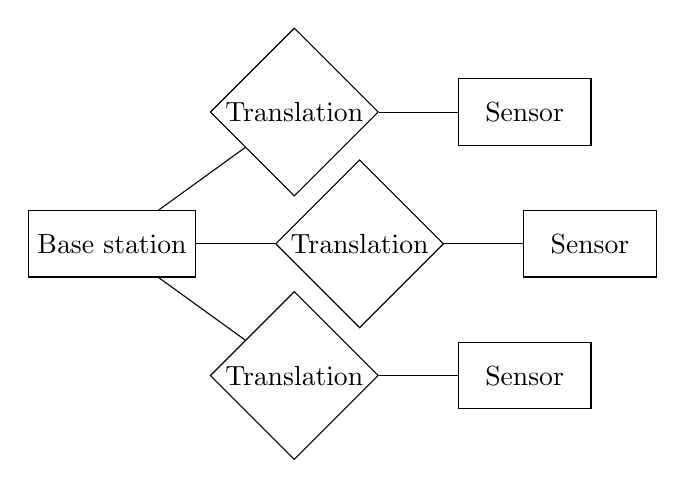
\begin{tikzpicture}[auto,node distance=1cm]
					\node[entity] (node1) {Base station}
									[grow=up,sibling distance=3cm];
					% Now place a relation (ID=rel1)
					\node[relationship] (rel1) [below right = of node1] {Translation};
					\node[relationship] (rel2) [right = of node1] {Translation};
					\node[relationship] (rel3) [above right = of node1] {Translation};
					% Now the 2nd entity (ID=rel2)
					\node[entity] (node2) [right = of rel1]	{Sensor};
					\node[entity] (node3) [right = of rel2]	{Sensor};
					\node[entity] (node4) [right = of rel3]	{Sensor};
					% Draw an edge between rel1 and node1; rel1 and node2
					\path (rel1) edge node {} (node1)
								edge	 node {}	(node2);
					\path (rel2) edge node {} (node1)
								edge	 node {}	(node3);
					\path (rel3) edge node {} (node1)
								edge	 node {}	(node4);
				\end{tikzpicture}
				\caption{Example connection diagram prototype}
			\end{figure}
			\paragraph{Prototype parts}
				\begin{enumerate}
					\item Base station
						\begin{enumerate}
							\item Wi-Fi accesspoint
							\item Web interface
							\item Recording
						\end{enumerate}
					\item Sensors
						\begin{enumerate}
							\item GPS
							\item Temperature and humidity sensor
							\item CO2 sensor (two types)
							\item Heart-rate sensor
							\item Galvanic skin response sensor
							\item Camera (PI-cam)
						\end{enumerate}
				\end{enumerate}
			\paragraph{Prototype features}
				The base station allows all sensors to be plugged and played while turned on except for the Pi-cam, this is either build in or it is not. Each sensor can be seen on the web interface or via the screen of the base station. The recordings can only be started via the touch screen on the base station. Recordings can be downloaded from the web interface or via USB stick that can be mounted on the base station. Every sensor is attached to the base station via USB for ease of use and availability of the devices. An USB hub can easily be used to extend the amount of sensors the base station can handle simultaneously. 
		\subsection{Bias}
			Bias is a risk that always occurs when doing research. To avoid bias the researchers have tried not to intervene with the test subjects and only guide them through the process. Only when necessary the researchers would share their point of view with the test subjects. Also during the processing of the outcome of the research and the test the researchers try to have a position as neutral as possible regarding to the topic that is being researched. Another measure taken is the selection of text-subjects. During the testing phase there are a few selected researchers from different backgrounds who applied, this way there is a diversity in the group of selected researchers. The group of students as test-subjects are also selected by their background to have group that is more diverse as only students with the same background. Because of this the bias is kept as minimal as possible with the resources available. It may had been totally absent but this would result in a project-duration longer than the given 10, or 20 when looking at the total project, weeks. We decided to use a fairly diverse group of test subjects, however the size of the group and the diversity could have been bigger by including more faculties.
		\subsection{Research}
			In this section is described how each sub question of our main research question is researched. So as to decide the effective method of research we have considered what we needed to do with the research. We considered what should be focused more between breadth and depth or between quantification and qualification and what would be more efficient in empirical research and desk research in each sub question. Along with these considerations, we have came to the following decision. 

			First, to research 'how technical are the students and researchers from the Makerslab on the Amsterdam University of applied sciences?', We let students and researchers from the Makerslab use the Monitoring box. Because we wanted to gain various types of students and researchers in technical point, panels of survey should be breadth. With this we can determine what explanation is needed according to the technical level. So, questions of survey include users' comments so to gain insight in to this. 

			Second, in order to research 'What improves the usability of the product when taking the structure plane of user experience into account?', surveys and desk research are used. And compare this with the shortcomings in usability aspects through existing, similar-functioning platforms and devices. In order to research the Monitoring box in the direction of improving the insufficient aspects of usability.

			Third, in order to research the question 'How can the data be made available such that the students \& researchers from the Minor Makerslab can use it?' desk research is used. We look at other similar cases and consider choosing the most appropriate way of data sharing and how researchers use open source and data gathering platforms.
		\paragraph{Interview setup} The interviews were executed in the following order:
			\begin{enumerate}
				\item \textbf{Give general introduction of project to participant.} \\
				Describe the goal, what we are researching and what we they are going to do.
				\item \textbf{Let participant assemble hardware and upload software.}\\
				Of the MonitoringBox. While he or she is doing the assembly of the prototype we observe participant.
				\item \textbf{Let the participant test their work.}\\
				By connecting the sensor to the Raspberry Pi and trying to record.
				\item \textbf{Let participant use the prototype.}\\
				So that the participant will use all the different features of the software and we observe them.
				\item \textbf{Ask participant questions from the survey and ask for general feedback.}\\
				Such to get structured information and really find out what they thought.
			\end{enumerate}
			The interviews were recorded with a camera and notes were made during this interview. All team members were present during the interviews, one member controlled the camera, one made notes and one did the presentation and guidance.
\section{Results}
		\begin{figure*}[ht]
			\centering
			\begin{tabular}{ | l | l | l | l | l | l | l | l | l | l | }
				\hline
							& 				& 		& Skill	& 		& 			& 		& 				& 		& 		\\ 
							& 				& 		& level	& Time	& Sensors	& Code 	& Knowledge		& Order & Web	\\ 
			Participant		& Study			& Age	& 1-10	& taken	& created	& error & gap issues	& issues& UI\\ \hline \hline
			Researcher A	& N.A.			& 30-35 & 4		& 81	& Humidity	& 		& 				& 		&		\\ 
							& 				& 		& 		& 		& CO2		& 		& 				& 		& 		\\ 
							& 				& 		& 		& 		& GPS		& 		& 				& 		& 		\\
							& 				& 		& 		& 		& GSR		& 		& 				& 		& 		\\
							& 				& 		& 		& 		& Heartrate	& 		& 				& 		& 		\\ \hline
			Researcher B	& N.A.			& 25-30 & 5 	& 52	& Humidity	& 		& 				& 		& 		\\ 
							& 				& 		& 		& 		& CO2		& 		& 				& 		& 		\\
							& 				& 		& 		& 		& GPS		& 		& 				& 		& 		\\
							& 				& 		& 		& 		& GSR		& 		& 				& 		& 		\\
							& 				& 		& 		& 		& Heartrate	& 		& 				& 		& 		\\ \hline
			Student A		& BIM	& 20-25 & 4 	& 25	& CO2 		& 		& 				& 		& 		\\
							& 				& 		& 	 	& 		& GPS		& 		& 				& 		& 		\\
							& 				& 		& 	 	& 		& GSR		& 		& 				& 		& 		\\ \hline
			Student B		& GD 			& 25-30 & 8 	& 32	& CO2		& 		& 				& 		& 		\\
							& 				& 		& 		& 		& GPS		& 		& 				& 		& 		\\
							& 				& 		& 		& 		& Humidity	& 		& 				& 		& 		\\
							& 				& 		& 		& 		& GSR		& 		& 				& 		& 		\\ \hline
			Student C		& DE			& 20-25 & 5		& 20	& CO2		& 		& 				& 		& 		\\ 
							& 				& 		& 		& 		& GPS		& 		& 				& 		& 		\\
							& 				& 		& 		& 		& Heartrate	& 		& 				& 		& 		\\ \hline
			Student D		& SE 			& 25-30	& 9		& 21	& Humidity	& 		& 				& 		& 		\\ 
							& 				& 		& 		& 		& GPS		& 		& 				& 		& 		\\ 
							& 				& 		& 		& 		& GSR		& 		& 				& 		& 		\\ \hline
			Student E		& BIM		 	& 20-25	& 5 	& 38	& Humidity	& 		& 				& 		& 		\\ 
							& 				& 		& 		& 		& GPS		& 		& 				& 		& 		\\ 
							& 				& 		& 		& 		& Heartrate	& 		& 				& 		& 		\\ \hline
			Student F		& SE 			& 20-25	& 8		& 39	& Humidity	& 		& 				& 		& 		\\ 
							& 				& 		& 		& 		& GPS		& 		& 				& 		& 		\\ 
							& 				& 		& 		& 		& CO2		& 		& 				& 		& 		\\ 
							& 			 	& 		& 		& 		& Heartrate& 		& 				& 		& 		\\ 
							& 				& 		& 		& 		& GSR		& 		& 				& 		& 		\\ \hline
			\end{tabular}
			\caption{General distribution of participants}
		\end{figure*}
		\begin{tabular}{ | l | l | }
			\hline
			Abriviation & Study 					\\ \hline \hline
			BIM			& Business It Management	\\ \hline
			GD			& Game Design				\\ \hline
			DE			& Design					\\ \hline
			SE			& Software Engineering		\\ \hline
		
		\end{tabular}
	\subsection{Interview participants}
		In order to get an accurate picture of the user group, a sample of users with different backgrounds were chosen. This included students and researchers with different levels of technical skills. The participants of the interviews can be categorized in to the following categories:
		\begin{figure}[ht]
			\centering
			\begin{tabular}{ | l | r | l | }
				\hline
				Type			& Amount	& Description \\ \hline \hline
				Researcher		& 2			& Different technical levels* \\ \hline
				Student			& 4			& See figure ... for details \\ \hline \hline
				Total			& 6			& \\ \hline
			\end{tabular}
			\caption{General distribution of participants}
		\end{figure}\\
		The student groups can be sub divided into different sub-categories:
		\begin{figure}[ht]
			\centering
			\begin{tabular}{ | l | r | l | }
				\hline
				Type					& Amount \\ \hline \hline
				Business IT				& 1 \\ \hline
				Game design				& 1 \\ \hline
				Software engineering	& 2 \\ \hline
				Total					& 4 \\ \hline
			\end{tabular}
			\caption{Major of the participating students}
		\end{figure} \\
		This shows a users from varying backgrounds participated in the research. However, unfortunately because of time and resources we had limitation in size of this group
		\begin{enumerate}
			\item How technical are the students and researchers from the Makerslab on the Amsterdam University of applied sciences?
				\begin{enumerate}
					\item What documentation is needed and how detailed should it be
				\end{enumerate}


				\begin{enumerate}
					\item Researcher A

						The researcher encountered the following problems during the interview.\\

						First, she does not know how to use a breadboard. To create a Galvanic Skin Response sensor, users have to connect the Arduino Nano, resistor, and several wires. However, these connections are not just one-to-one connections, they require multiple connections. So in order to succeed, users must understand the structure of the breadboard. The manual did not explain the structure of the breadboard, and the researcher had difficulty with it.\\
						Second, she wanted more specify information about cable connections.\\
		 		
						The researcher has mentioned that we need the following elements in the document.\\

						First, she suggested that we mention in the manual how to use breadboard and the structure of breadboard. \\
						Second, she suggested that we add more information about Arduino nano and Arduino uno.\\
						Third, she said the manual does not focus in Dutch, but English. \\
		
					\item Researcher B

						Researcher B knows quite a bit of software and has little knowledge of hardware. The researcher encountered the following problems during the interview.\\

						First, he feels there are something unclear about the schematic. 						He pointed out that the schematic pin number is missing. The pin number is too small to specify, so he was uncomfortable with rebuilding.\\
						Second, he was wondering about the difference between the two CO2 sensors. The manual only briefly specifies the name and characteristics of each sensor, but the difference between the two sensors is not specified in detail.\\
						Third, he did not know how to use the breadboard.\\

						The researcher has mentioned that we need the following elements in the document.\\

						First, he suggested that we mention in the manual when to upload and where to see the results. \\
						Second, he suggested links to tutorials about breadboard.\\
						Third, he suggested that we put the technical names in the shopping list\\
						Forth, he suggested that we explain in the manual which part is wrong for each error message.\\

					\item Student A

						Student A is majoring in Software engineering and has  quite some experience in Arduino. The student A encountered the following problems during the interview.\\

						First, he was confused about the GPS and Arduino nano. He was confused because the GPS and Arduino nano have similar size and similar color.\\
						Second, he had difficulty reading the schematics. The letters in the schematics are too small to read, and it took some time to find out what was written on the next page.\\

						The researcher has mentioned that we need the following elements in the document.\\

						First, he suggested to write the steps in the manual in a bold font.\\
						Second, he suggested adjusting the order of text and schematics. He mentioned that it took a some time to find that there is a text which explain schematics. 

					\item Student B

						Student B is majoring in Game development and has  quite some experience in Arduino. He replied that his technical level is a hobby in the hardware and professional in the software. The student B pointed out the following during the interview.\\

						First, the manual is really easy but it did not state which Arduino sketch is necessary to complete.
						Second, pictures should represent the real life device. Heart rate sensor in the schematics and the real heart rate sensor look different.

					\item Student C

						Student C is majoring in Software engineering and has  quite some experience in Arduino. The student C pointed out the following during the interview.\\

						First, the Galvanic Skin Response schematic is not clear. The Galvanic Skin Response chapter is not in depth with the explanation of how to connect everything.\\
						Second, he ask how can he test the sensors.\\
						Third, he suggested that we explain more information about cable.\\

					\item Student D

						Student D is majoring in Business IT. He has understanding of user software like programs on window and can read code but not make it. The student D pointed out the following during the interview.\\

						First, it is unclear how the wires are connected.\\
						Second, the chapter order is not good. He recommended put the pushing code chapter be after connecting the wires.\\
						Third, the soldering is hard so the breadboard should be shown.\\
						Forth, he suggested that we show how the arduino and computer are connected while pushing.\\
	
						He said the Manual is pretty clear but it is not detailed enough. It is unclear where a button is and when he have to upload software. And he suggested that we describe some failures and add 3D photographs. So He thought students with similar levels can have some trouble. 
				\end{enumerate}

			\item What improves the usability of the product when taking the structure plane of user experience into account?

				In interaction design in the structure plane of user experience, users must communicate correctly to the monitoring box and the monitoring box must deliver the information that the user wants immediately and accurately. In this respect, the Monitoring box has a touch screen and we have added four menus in this screen so that when the user has the information they want, they can instantly check the menu. The home screen shows what percentage of the storage capacity is in use and if users select 'Sensor' menu from the Monitoring Box, users can see the currently connected sensor. And if users select 'Wi-Fi' menu from Monitoring Box, users can confirm the Wi-Fi name and password.//
				In information architecture in the structure plane of user experience, it should facilitate intuitive access to data. So we used wireless Wi-Fi so that we could check the information if we had an internet capable device. And with a single push of a button on the Internet Web site, users are able to download the data of the sensors they had recorded at a glance. In addition, the monitoring box screen design allows intuitive use of the menu.
\\

			\item How can the data be made available such that the students \& researchers from the Minor Makerslab can use it?
				\begin{enumerate}
					\item In the Monitoring Box
				\begin{enumerate}
			\item Screen
				\begin{enumerate}
					\item Main menu

						In the main menu, there is one bar and four menus. The bar tells users how much storage they have used. This percentage allows the user to see how much memory is left on the SD card and to control usage. Each menu button has a label for explaining its purpose.\\
					\item Record

						Users can start recording by pushing this menu. In addition, they can see which sensors are recording while recording.\\
					\item Sensor

						In the Sensor menu, users can see a list of currently connected sensors. It is good to check before users know that the users are sure of the connection.\\
					\item Wi-Fi

						Wi-Fi name and password can be found in this menu. Users do not need to remember or write down the Monitoring Box its Wi-Fi name and password.\\
				\end{enumerate}
			\end{enumerate}
		\item On the Website
			\begin{enumerate}
				\item Wireless connecting to Web page

					The data that users have recorded can be downloaded at once. We use the wireless data transmitter to view the data, even if users do not have a certain cable, users can see data only if they have a Wi-Fi enabled devices such as a laptop, a computer or a smart phone. \\
					A few simple steps are required for users to connect their Monitoring Box to the Web page. First, turn on a Wi-Fi enabled devices and connect the Monitoring box to the Wi-Fi. The Monitoring box is equipped with a Wi-Fi function and the Wi-Fi name and password can be found in the menu on the monitoring box its screen. Then, after you completed the first step, users can go to the monitoring box its website by typing 'monitoring.box:5000' in as a website address.\\

				\item Download the recorded information

					After users access the website, they can see and download the data which they have recorded. The downloadable format is CSV(Comma Separated Value). Because it is truncated in the form of a comma, it can be read not only as a text file but also as an Excel file. When users open CSV file in Excel, the user can view and store the sorted data in sequence.\\

				\item Graph

					Users can view a list of currently connected sensors in real time on the web page and a graph of their sensor values. Users can easily access data and see the data at a glance.\\
			\end{enumerate}
		\end{enumerate}
 	\end{enumerate}
\section{Conclusion}
	This has no content yet or is a work in progress and thus not yet shown.

\section{Discussion}
	Looking at the main research question you may say that there is a variety of factors that contribute to the successful creation of an open source, multi-research, sensor geolocation aware, data gathering platform that can be used by the students and researchers from the Makerslab on the Amsterdam University of Applied Sciences. The usability is different for every device and modification of a device. Slight alternations may result in a total different user experience and the usability aspects. \\
	As there are not much projects similar to this project the main difference shows that this project has no 'custom made' items. Everything can be bought as separate parts from different suppliers. Though this requires some extra work it provides a higher certainty of availability. \\
	It could be said that this report and the results of the research only apply to the Monitoring Box. This is partially true, though any researcher or developer well informed about the topic they are going to research for can determine what results may apply to their product and what may not.

\section{Limitations}
	This has no content yet or is a work in progress and thus not yet shown.

\bibliographystyle{plain}
\bibliography{Research_Report_Monitoring_Box_IEEE_Style}

\end{document}